\documentclass[11 pt,oneside,a4paper,titlepage]{article}
\usepackage{preamble}
\renewcommand{\familydefault}{\sfdefault}
\graphicspath{{img/}}

\begin{document}

\sidebar{sideBarColor!25}
\SimpleHeader{titleBackColor}{Luca}{Olivieri}{Software Developer}{white}

% Side bar
\vspace*{3.49cm} % start 8 cm from the top of the page}
\adjustbox{valign=t}{
\begin{minipage}{7.3cm} % large 7.3 cm from the top
\vspace*{1.2cm} % text starts 1cm under the top of the minipage
	% Picture
	\begin{center}
	\begin{tikzpicture}
		\node[
		circle,
		minimum size=\cvPictureWidth,
		path picture={
		\node at (path picture bounding box.center){
			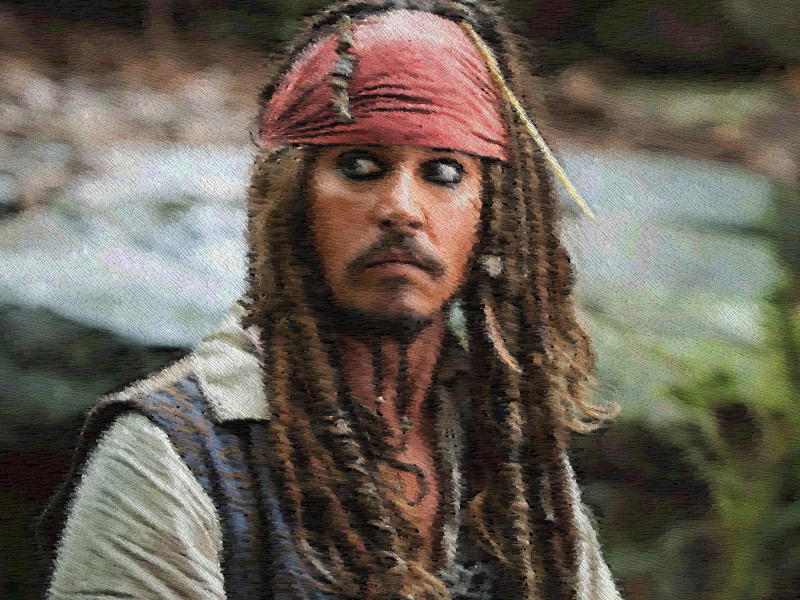
\includegraphics[width=\cvPictureWidth]{Picture.jpg}
			};
			}]
		{};
	\end{tikzpicture}
	\end{center}
	% In brief
	\ruleline{\textbf{About me}}
	I like to constantly challenge myself with learning new skills 
	and with personal projects, not always tech-related. 
	
	My first interest is programming, while electronics is my second one, preferably digital than analog. 

	My core value is to respect my work and the people I work with with.  
	% Contact
	\ruleline{\textbf{Contact}}
	\begin{tikzpicture}[every node/.style={inner sep=0pt, outer sep=0pt}]
	\matrix [
	column 1/.style={anchor=center,contactIcon},
	column 2/.style={anchor=west,align=left,contactIcon},
	column sep=5pt,
	row sep=5pt] (contact) {
	\node{\faEnvelope}; 
		& \node{\href{mailto:olivieri.luca@outlook.com}{olivieri.luca@outlook.com}};\\
	\node{\faPhone}; 
		& \node{+39 349 28 99 132};\\ 
	\node{\faMapMarker}; 
	& \node{Chiavari (GE), Italy};\\
	\node{\faLinkedinSquare}; 
	& \node{\href{https://www.linkedin.com/in/luca-olivieri-00714684/}{LinkedIn}};\\
	\node{\faInstagram}; 
	& \node{\href{https://www.instagram.com/olimexsmart/}{Instagram: @olimexsmart}};\\
	\node{\faGithub}; 
	& \node{\href{https://github.com/olimexsmart}{GitHub: @olimexsmart}};\\
	\node{\faCar};
	& \node{Driving License A and B};\\
		};
	\end{tikzpicture} 
    % Professional Skills 
    \ruleline{\textbf{Skills}}
    \begin{center}
        \cvtag{C}\cvtag{JS}\cvtag{Python}\cvtag{MatLab}\cvtag{C++}\cvtag{C\#}\cvtag{Git}
		\cvtag{CAD (basic)}\cvtag{\LaTeX}
    \end{center}
	% Languages
	\ruleline{\textbf{Languages}}
	\begin{tikzpicture}[every node/.style={inner sep=0pt, outer sep=0pt}]
	\matrix [
	column 1/.style={anchor=center,contactIcon},
	column 2/.style={anchor=west,align=left,contactIcon},
	column sep=5pt,
	row sep=5pt] (contact) {
	\node{\flag{Italy.png}};
	& \node{Italian - Native Language};\\
	\node{\flag{England.png}};
	& \node{English - Professional Knowledge};\\
	\node{\flag{CzechRep.png}};
	& \node{Czech - Basic Knowledge};\\
	};
	\end{tikzpicture} 
	% QR Code
	\begin{center}
		
\includegraphics[width=3.5cm]{QR_Info.png}
	\end{center}
\end{minipage}} %
\hfill 
% MAIN SECTION
\adjustbox{valign=t}{\begin{minipage}{11.3cm}
	% Work Experience
	\vspace*{1cm}
	\section*{{\faSuitcase} WORK EXPERIENCE}
	\MySectionNoPic{2021-2022}{Embedded System Developer}{Chiavari, Italia}{Hi-Lex Italy}
	{
		Microcontroller C programming for automotive and assembly line applications.
		Core developer for Jeep Avenger (J516) window lifter project.
		Development from the ground up of a desktop application in ElectronJS for debugging based on UART. 
		Kicked off Hardware-In-The-Loop testing with Robot Framework (Python). 
		Creation of automated signal generation and testing with MatLab and Simulink. 
		Re-organized Git workflow and setup of an on-premise GitLab instance running on Docker. 
		Assistance in electronic design. 
		Interfacing with MCU supplier on a day-to-day basis.
	}  

	\vspace*{0.22cm}
	\MySectionNoPic{2020-2021}{High School Teacher}{Sestri Levante}{Natta DeAmbrosis}
	{
		Programming, Electronics, IT
	}  

	\vspace*{0.22cm}
	\MySectionNoPic{2019-2020}{PhD in Legged Locomotion}{Trento}{University of Trento}
	{
		High performance C++ linear algebra. Optimization techniques. 
		Publications: \textit{"Fast and Accurate Multi-Body Simulation with Stiff Viscoelastic Contacts"}. 
		Teaching assistant in bachelor C++ programming courses. PhD interrupted at start of second year.
	}

	\vspace*{0.22cm}
	\MySectionNoPic{2019}{Full Stack Web Developer}{Genoa}{Deloitte}
	{
		Business to Business Internet of Things, both industrial and connected products. 
		Mainly back-end in Java Spring-Boot, building microservices in Cloud Foundry. 
		Front-end with Angular. 
	} 

	\vspace*{0.22cm}
	\MySectionNoPic{2017}{Backend Developer}{Chiavari}{Mainsim}
	{
		Paid internship. Full stack web developing, database and system management. 
		One-page application in jQuery, PHP and MySQL. Both Windows and Unix servers.
	}	

	% Education
	\section*{{\faGraduationCap} EDUCATION}

	\MySectionNoPic{2016-2018}{Master's Robotics Engineering}{Genoa}{University of Genoa}
	{
		Real-Time, concurrent and embedded programming. 	
		Modelling and control of robotic platforms, Machine Learning, Artificial Intelligence, 
		Computer Vision, ROS, POSIX. 

		Thesis: \emph{"Hybrid indoor localization for industrial AGVs".}

		Development from the ground-up of a segmentation algorithm and an Extended Kalman Filter 
		for an indoor localization system based on a laser scanner sensor. 
		Development in C++ in a Unix environment.
	}
		
	\vspace*{0.22cm}
	\MySectionNoPic{2016-2018}{Bachelor's Electronics Engineering and Information Technology}{Genoa}{University of Genoa}
	{
		Programming, Control Systems, Telecommunication Systems, Digital and Analog Electronics.
		
		Thesis: \emph{"Source Contact Graph Routing on a Nanosat network".} 

		Formulation of an a-priori routing algorithm for a satellite network. 
		C++ with NS3 network simulation package on Unix environment.
	}
\end{minipage}} %

%%%%%%%%%%%%%%%%%%%%%%%%%%%%%%%%%%%%%%%%%%%%%%%%%%%%%%%%%%%%
% Second Page
\newpage

\sidebar{sideBarColor!25}
\newpageheader{titleBackColor}{Jack}{Sparrow}{Pirate \faLightbulbO \hspace{1mm} Captain}{white}

% %%%%%%%%%%%%%%%%%%%%%%%%%%%%%%%%%% SIDEBAR %%%%%%%%%%%%%%%%%%%
\adjustbox{valign=t}{%
\begin{minipage}{7.3cm} 
\vspace*{0.4cm} % text starts 0.4cm under the top the header


        
    %%%%%%%%%%%%%%%%%%%%%%%%%%%%%%%%%%%%%%%%%%%%%%%%%%%%
    % Skill and Strengths 
    \ruleline{\textbf{Soft Skills and Strengths}}
    \vspace*{-0.5cm}
    \begin{center}
        \cvtag{Creativity}\cvtag{Curiosity}\cvtag{Flexibility}\cvtag{Self Confidence}\cvtag{Ability to Plan and Organize} \cvtag{Autonomy}\cvtag{Adaptability} \cvtag{Eye for Details}\cvtag{Problem Solving}\cvtag{Team Working}\cvtag{Love Learning New Things}\cvtag{Leadership}\cvtag{Good Communication}\cvtag{Managing Information}\cvtag{Diplomacy}\cvtag{Good Listener}\cvtag{Patience}
    \end{center}

    %%%%%%%%%%%%%%%%%%%%%%%%%%%%%%%%%%%%%%%%%%%%%%%%%%%%
    % Professional Skills 
    \ruleline{\textbf{Professional Skills}}
    \begin{center}
        \cvtag{Skill 1}\cvtag{Skill 2}\cvtag{Skill 3}\cvtag{Skill 4}\cvtag{Skill 5}
    \end{center}

    %%%%%%%%%%%%%%%%%%%%%%%%%%%%%%%%%%%%%%%%%%%%%%%%%%%
    % Other Interests
    \ruleline{\textbf{Other Interests}}
    \small
    \begin{multicols}{2}
        \begin{itemize} 
            \item  Guitar \flag{Guitar.png}
            \item  Piano \flag{Piano.png}
            \item  Chess \flag{Chess.png}
            \item  Gym \flag{Gym.png}
            \item  Travels \flag{Travels.png}
            \item  Movies \flag{movie2.png}
            \item  Books \flag{Books.png}
    \end{itemize}
    \end{multicols}

     %%%%%%%%%%%%%%%%%%%%%%%%%%%%%%%%%%%%%%%%%%%%%%%%%%%%%
        % QR Code
        \ruleline{\textbf{Download My CV}}
        \scriptsize
        \centering
        Download my CV via the QR below \aiOverleaf.
        \begin{center}
            \quad
            \qrcode[height=2cm]{
                https://www.dropbox.com/sh/k5pheguf9jrur8x/AADpyjYJi7V5bhPyJeP3H74ea?dl=0} \\
            \vspace*{0.5cm}
        \end{center}

\end{minipage}
}%
\hfill
%%%%%%%%%%%%%%%%%%%%%%%%%%%%%%%%%%% MAIN %%%%%%%%%%%%%%%%%%%%%%%%%
\adjustbox{valign=t}{%
\begin{minipage}{11.3cm}
    \vspace*{0.4cm}

    \section*{{\aiOBP} About me}
    Programming in general is my first interest, constantly challenging myself with new ideas and projects. My programming projects range from high level GUI application like an Android app (Olmaredo Stego) to embedded projects like an OBD2 telemetry interface for cars. Recently I've started to look into the Flutter framework, while at Hi-Lex I've been developing a fairly complex desktop application in Electron.
    
    Electronics is my second interest, preferably digital than analog. More in detail, I developed several complex Arduino projects and experimented with the STM32 microcontroller ecosystem. At Hi-Lex the core product is based on a Melexis MCU, very challenging both from the point of view of the resources available and the development environment.
    
    During my internship at Mainsim I first learned about web developing, mainly back-end but a with a touch of front-end too. This new set of skills allowed me to dive into the IoT paradigm that was when the core focus of the work in Deloitte.
    
    While in my PhD experience, although not completed, thought me about complex algebraic computation in Python and C++, up to that point my coding was approached in a results ASAP approach. My recent experience in the automotive industry instead made me completely re-think my day-to-day work and the implications of my coding for the company, forcing me to focus instead on the solidity of the product, shifting to a writing less code but of high quality.
    
    Finally, I try to keep my pragmatic approach fresh by 


    %%%%%%%%%%%%%%%%%%%%%%%%%%%%%%%%%%%%%%%%%%%%%%%%%%%
    % Peer Reviews
    % \section*{{\faBook} ACADEMIC PEER REVIEWS}
    % \footnotesize I did academic peer review for the following journals: 
    % \begin{itemize}
    %     \footnotesize
    %      \item{\textbf{Scientific Piracy}, IF: 4.996 (1720), September 1720;}
    %  \end{itemize}
        
    %%%%%%%%%%%%%%%%%%%%%%%%%%%%%%%%%%%%%%%%%%%%%%%%%%%
    % Information Technology Skills
    \section*{{\faDesktop} INFORMATION TECHNOLOGY SKILLS}
    
    \ITCcompetence{Data Analysis}{
    \textbf{MATLAB}: \textit{Higly Specialized}\\
    \textbf{Wolfram Mathematica}: \textit{Intermediate}\\
    \textbf{Jupiter Notebook}: \textit{Intermediate}\\
    }
    
    \vspace*{0.22cm}

    \ITCcompetence{Modeling and Simulation}{
    \textbf{Simulink} : \textit{Intermediate}  \\
    \textbf{LTSpice}: \textit{Intermediate}
    }
    
    \vspace*{0.22cm}

    \ITCcompetence{Audio Processing}{
    \textbf{Reaper} : \textit{Advanced}  \\
    }

    \vspace*{0.22cm}

    \ITCcompetence{Office Automation}{
    \textbf{MS Office (Excel, Word, PowerPoint)}: \textit{Higly Specialized}\\
    \textbf{\LaTeX}: \textit{Advanced}\\
    }
    
    %%%%%%%%%%%%%%%%%%%%%%%%%%%%%%%%%%%%%%%%%%%%%%%%%%%
    % Programming Languages
    \section*{{\faCode} PROGRAMMING LANGUAGES}
    \vspace*{-0.5cm}
    \begin{multicols}{2}    
    \begin{itemize}
    \footnotesize
        \item \textbf{Matlab}: Highly Specialised
        \item \textbf{Python}: Advanced
        \item \textbf{SQL}: Intermediate
        \item \textbf{C/C++}: Intermediate
        \item \textbf{Java}: Basic
        \item[\vspace{\fill}]
    \end{itemize}
    \end{multicols}
    
    %%%%%%%%%%%%%%%%%%%%%%%%%%%%%%%%%%%%%%%%%%%%%%%%%%%
    % Certificates
    \section*{{\faCertificate} CERTIFICATES}
    
    \adjustbox{valign=t}{\begin{minipage}{2cm}
    \begin{center}
        
\includegraphics[width=1.2cm]{IBM.png}
    \end{center}
    \end{minipage}}
    \hfill \vline \hfill
    \adjustbox{valign=t}{\begin{minipage}{9cm}
        \begin{itemize}
            \scriptsize 
            \item Python for Data Science, AI \& Development (\textit{Coursera, 2022})
        \end{itemize}
    \end{minipage}}
    
    \vspace*{0.2cm}
    
    \adjustbox{valign=t}{\begin{minipage}{2cm}
    \begin{center}
        
\includegraphics[width=2cm]{Matlab.png}
    \end{center}
    \end{minipage}}
    \hfill \vline \hfill
    \adjustbox{valign=t}{\begin{minipage}{9cm}
        \begin{itemize}
            \scriptsize 
            \item Pirate Processing with MATLAB (\textit{Mathworks, 2022})
            \item Signal Processing with MATLAB (\textit{Mathworks, 2022})
            \item Deep Learning with MATLAB (\textit{Mathworks, 2022})
            \item Machine Learning with MATLAB (\textit{Mathworks, 2021})
        \end{itemize}
    \end{minipage}}
    
    \vspace*{0.2cm}
    
    \adjustbox{valign=t}{\begin{minipage}{2cm}
    \begin{center}
        
\includegraphics[width=1.2cm]{google.png}
    \end{center}
    \end{minipage}}
    \hfill \vline \hfill
    \adjustbox{valign=t}{\begin{minipage}{9cm}
        \begin{itemize}
            \scriptsize 
            \item How to became a Web Pirate (\textit{Google Pirate School, 2022})
            \item item 2
            \item item 3
            \item item 4
        \end{itemize}
    \end{minipage}}
    
    \vspace*{0.2cm}
    
\end{minipage}}


\end{document}
